% ============================================================================
%  FIRST DOCUMENTATION --- Project Overview \& Output Showcase
%  Cloud-Native AI Operations Agent for CEM--CVM Intelligence
%  Souhayl Guenichi | ESPRIT | Huawei Tunisia | March 2026
% ============================================================================
\documentclass[12pt,a4paper]{report}

% -- Packages ----------------------------------------------------------------
\usepackage[utf8]{inputenc}
\usepackage[T1]{fontenc}
\usepackage[english]{babel}
\usepackage[top=2.2cm,bottom=2.2cm,left=2.5cm,right=2.5cm]{geometry}
\usepackage{lmodern}
\usepackage{microtype}
\usepackage{graphicx}
\usepackage[dvipsnames,svgnames,x11names]{xcolor}
\usepackage{tikz}
\usetikzlibrary{
  shapes.geometric,arrows.meta,positioning,fit,calc,
  backgrounds,shadows,decorations.markings,matrix,
  patterns,chains,scopes
}
\usepackage{pgfplots}
\pgfplotsset{compat=1.18}
\usepackage{booktabs}
\usepackage{tabularx}
\usepackage{multirow}
\usepackage{longtable}
\usepackage{array}
\usepackage{listings}
\lstset{
  basicstyle=\ttfamily\footnotesize,
  keywordstyle=\color{RoyalBlue}\bfseries,
  commentstyle=\color{ForestGreen}\itshape,
  stringstyle=\color{Crimson},
  backgroundcolor=\color{gray!5},
  frame=single, rulecolor=\color{gray!40},
  breaklines=true, numbers=left, numberstyle=\tiny\color{gray},
  tabsize=2, showstringspaces=false, captionpos=b,
}
\usepackage{amsmath,amssymb}
\usepackage[colorlinks=true,linkcolor=RoyalBlue,citecolor=ForestGreen,urlcolor=Crimson,
  pdfauthor={Souhayl Guenichi},
  pdftitle={AI Operations Agent -- First Documentation}]{hyperref}
\usepackage{bookmark}
\usepackage{fancyhdr}
\pagestyle{fancy}\fancyhf{}
\fancyhead[L]{\nouppercase{\leftmark}}
\fancyhead[R]{\thepage}
\renewcommand{\headrulewidth}{0.4pt}
\usepackage[font=small,labelfont=bf]{caption}
\usepackage{subcaption}
\usepackage{enumitem}
\usepackage{float}

% -- Colors ------------------------------------------------------------------
\definecolor{huaweired}{HTML}{CF0A2C}
\definecolor{huaweidark}{HTML}{1A1A2E}
\definecolor{ossblue}{HTML}{2E86AB}
\definecolor{bssgreen}{HTML}{2ECC71}
\definecolor{aiviolet}{HTML}{8E44AD}
\definecolor{cvmorange}{HTML}{E67E22}
\definecolor{cemteal}{HTML}{1ABC9C}
\definecolor{datalake}{HTML}{3498DB}
\definecolor{darkbg}{HTML}{2C3E50}
\definecolor{lightgray}{HTML}{ECF0F1}
\definecolor{actionred}{HTML}{E74C3C}

% -- TikZ Styles -------------------------------------------------------------
\tikzset{
  service/.style={rectangle,rounded corners=4pt,minimum width=2.8cm,minimum height=1cm,
    draw=#1!70!black,fill=#1!15,text=black,font=\small\bfseries,
    drop shadow={shadow xshift=0.8pt,shadow yshift=-0.8pt,opacity=0.12},
    align=center,line width=0.7pt},
  service/.default={ossblue},
  datastore/.style={cylinder,shape border rotate=90,aspect=0.25,
    minimum width=2cm,minimum height=1.2cm,
    draw=#1!70!black,fill=#1!12,text=black,font=\small\bfseries,
    align=center,line width=0.7pt},
  datastore/.default={datalake},
  external/.style={rectangle,rounded corners=2pt,minimum width=2.4cm,minimum height=0.8cm,
    draw=gray!60,fill=gray!8,text=black,font=\small,dashed,align=center,line width=0.6pt},
  myarrow/.style={-{Stealth[length=5pt]},line width=0.8pt,#1},
  myarrow/.default={darkbg},
  biarrow/.style={{Stealth[length=4pt]}-{Stealth[length=4pt]},line width=0.7pt,#1},
  biarrow/.default={darkbg},
  arrlabel/.style={font=\scriptsize,fill=white,inner sep=1pt,text=darkbg},
}

% =============================================================================
\begin{document}

% -- TITLE PAGE ---------------------------------------------------------------
\begin{titlepage}
\begin{center}
\vspace*{1cm}
{\large\textsc{ESPRIT --- \'Ecole Sup\'erieure Priv\'ee d'Ing\'enierie et de Technologies}}\\[3pt]
{\small Department of Computer Science and Telecommunications}\\[0.8cm]
{\small In partnership with}\\[3pt]
{\large\textsc{Huawei Tunisia --- Cloud IT / Sales-Solution}}

\vspace{1.5cm}
\rule{\linewidth}{0.8pt}\\[0.5cm]
{\LARGE\bfseries Cloud-Native AI Operations Agent\\[6pt] for CEM--CVM Intelligence}\\[0.3cm]
{\large\itshape First Documentation --- Project Overview \& Deliverables}\\[0.3cm]
\rule{\linewidth}{0.8pt}

\vspace{1.5cm}
{\large\textbf{End-of-Studies Project (PFE)}}\\[0.3cm]
{\large Engineering Degree in Computer Science / Telecommunications}

\vspace{1.2cm}
\begin{tabular}{rl}
\textbf{Student:}      & Souhayl Guenichi \\[3pt]
\textbf{Host Company:} & Huawei Tunisia --- Cloud IT / Sales-Solution \\[3pt]
\textbf{Academic Year:}& 2025--2026 \\
\end{tabular}

\vfill
{\small March 2026}
\end{center}
\end{titlepage}

% -- TABLE OF CONTENTS --------------------------------------------------------
\tableofcontents
\newpage

% =============================================================================
%  CHAPTER 1 --- PROJECT OVERVIEW
% =============================================================================
\chapter{Project Overview}

\section{The Problem}

Telecom operators generate massive volumes of data across two historically siloed domains:

\begin{itemize}[nosep]
  \item \textbf{OSS (Operations Support Systems):} Network KPIs --- throughput, latency, packet loss, signal strength, cell load --- monitored per cell tower, per time window.
  \item \textbf{BSS (Business Support Systems):} Subscriber metrics --- revenue, data usage, voice minutes, churn risk, ARPU --- tracked per subscriber, per billing period.
\end{itemize}

\noindent When a cell degrades, operations teams detect it through KPI alarms. But the business team only sees the revenue impact days later. \textbf{No system automatically bridges network quality and business outcome, and no system takes autonomous action to prevent revenue loss.}

\section{The Solution}

We built a \textbf{Cloud-Native AI Operations Agent} --- an autonomous intelligence layer between Huawei's CEM (Customer Experience Management / SmartCare) and CVM (Customer Value Management). Unlike passive analytics platforms, our agent \textbf{detects, decides, and acts}:

\begin{enumerate}[nosep]
  \item \textbf{Detects} anomalies in both network and revenue streams using ML models.
  \item \textbf{Decides} by correlating OSS and BSS data, scoring SLA risk, and evaluating business impact.
  \item \textbf{Acts} by autonomously generating actionable recommendations: churn prevention campaigns, proactive network alerts, upsell triggers for healthy segments, and escalation tickets for critical incidents.
\end{enumerate}

\begin{figure}[H]
\centering
\resizebox{\textwidth}{!}{%
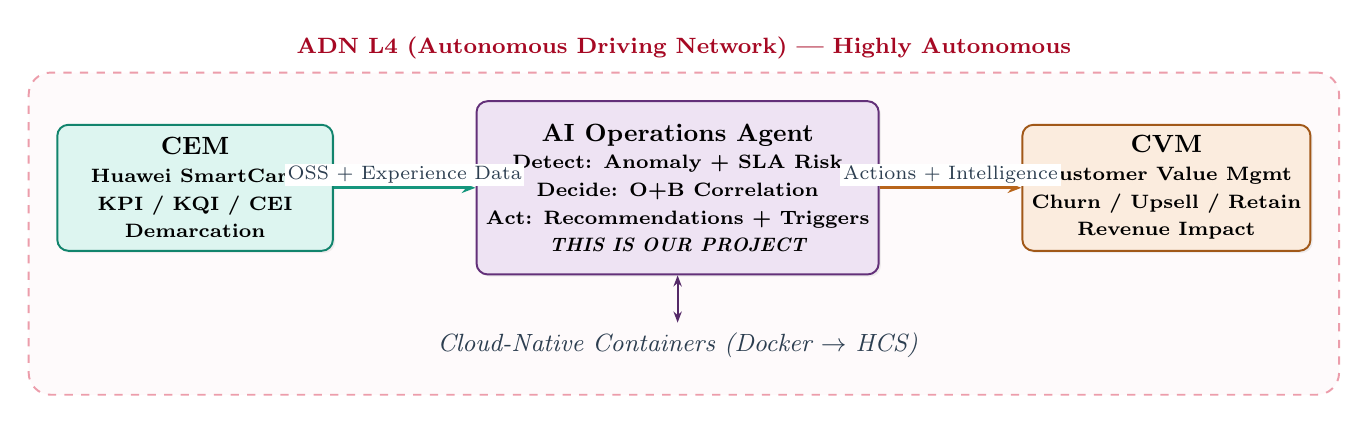
\begin{tikzpicture}[node distance=1.8cm]
  \node[service=cemteal,minimum width=3.5cm,minimum height=1.6cm] (cem) {
    \textbf{CEM}\\[-1pt]{\scriptsize Huawei SmartCare}\\[-1pt]
    {\scriptsize KPI / KQI / CEI}\\[-1pt]{\scriptsize Demarcation}};
  \node[service=aiviolet,minimum width=5cm,minimum height=2.2cm,right=of cem] (agent) {
    \textbf{AI Operations Agent}\\[-1pt]{\scriptsize Detect: Anomaly + SLA Risk}\\[-1pt]
    {\scriptsize Decide: O+B Correlation}\\[-1pt]
    {\scriptsize Act: Recommendations + Triggers}\\[-1pt]
    {\scriptsize\bfseries\itshape THIS IS OUR PROJECT}};
  \node[service=cvmorange,minimum width=3.5cm,minimum height=1.6cm,right=of agent] (cvm) {
    \textbf{CVM}\\[-1pt]{\scriptsize Customer Value Mgmt}\\[-1pt]
    {\scriptsize Churn / Upsell / Retain}\\[-1pt]{\scriptsize Revenue Impact}};
  \node[below=0.6cm of agent,font=\small\itshape,text=darkbg] (cloud) {
    Cloud-Native Containers (Docker $\to$ HCS)};
  \draw[myarrow=cemteal!80!black,line width=1pt] (cem) -- (agent)
    node[arrlabel,midway,above] {OSS + Experience Data};
  \draw[myarrow=cvmorange!80!black,line width=1pt] (agent) -- (cvm)
    node[arrlabel,midway,above] {Actions + Intelligence};
  \draw[biarrow=aiviolet!60!black] (agent) -- (cloud);
  \begin{scope}[on background layer]
    \node[fit=(cem)(agent)(cvm)(cloud),inner sep=10pt,
      draw=huaweired!40,dashed,rounded corners=8pt,fill=huaweired!2,line width=0.7pt] (adn) {};
  \end{scope}
  \node[above=1pt of adn.north,font=\footnotesize\bfseries,text=huaweired!80!black] {
    ADN L4 (Autonomous Driving Network) --- Highly Autonomous};
\end{tikzpicture}}%
\caption{Industrial positioning: CEM $\to$ AI Agent $\to$ CVM within ADN L4.}
\label{fig:positioning}
\end{figure}

\section{Key Differentiators}

\begin{enumerate}[nosep]
  \item \textbf{Autonomous Agent, Not Passive Analytics} --- The system detects, decides, and acts. It generates CVM-ready action recommendations autonomously, with human oversight only for critical escalations.
  \item \textbf{Real Operator Data} --- Trained on anonymised production data from Tunisie Telecom (not synthetic).
  \item \textbf{O+B Convergence} --- Statistically correlates network degradation with business impact (Pearson + Spearman).
  \item \textbf{Cloud-Native \& HCS-Portable} --- 5 Docker containers, directly mappable to Huawei Cloud Stack.
  \item \textbf{ADN L4 Positioning} --- Implements Level 4 (Highly Autonomous) of Huawei's Autonomous Driving Network: AI decides and acts, humans handle edge cases only.
\end{enumerate}

% =============================================================================
%  CHAPTER 2 --- ARCHITECTURE
% =============================================================================
\chapter{System Architecture}

\section{Container Architecture (5 Services)}

\begin{figure}[H]
\centering
\resizebox{\textwidth}{!}{%
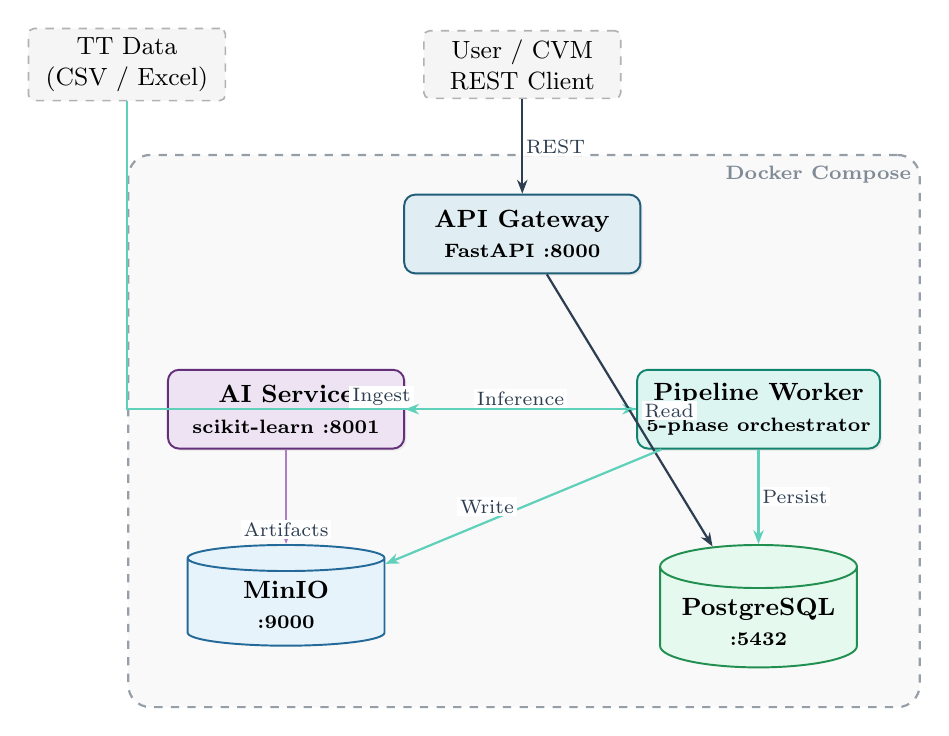
\begin{tikzpicture}[node distance=1.2cm and 1.8cm]
  \node[external,minimum width=2.5cm] (user) {User / CVM\\REST Client};
  \node[external,minimum width=2.5cm,left=2.5cm of user] (ttdata) {TT Data\\(CSV / Excel)};
  \node[service=ossblue,below=1.2cm of user,minimum width=3cm] (apigw) {
    \textbf{API Gateway}\\{\scriptsize FastAPI :8000}};
  \node[service=aiviolet,below=of apigw,minimum width=3cm,xshift=-3cm] (ai) {
    \textbf{AI Service}\\{\scriptsize scikit-learn :8001}};
  \node[service=cemteal,below=of apigw,minimum width=3cm,xshift=3cm] (worker) {
    \textbf{Pipeline Worker}\\{\scriptsize 5-phase orchestrator}};
  \node[datastore=datalake,below=1.2cm of ai,minimum width=2.5cm] (minio) {
    \textbf{MinIO}\\{\scriptsize :9000}};
  \node[datastore=bssgreen,below=1.2cm of worker,minimum width=2.5cm] (pg) {
    \textbf{PostgreSQL}\\{\scriptsize :5432}};
  \begin{scope}[on background layer]
    \node[fit=(apigw)(ai)(worker)(minio)(pg),
      draw=darkbg!50,fill=darkbg!3,rounded corners=8pt,inner sep=14pt,
      line width=0.8pt,dashed] (docker) {};
  \end{scope}
  \node[below=1pt of docker.north east,anchor=north east,
    font=\scriptsize\bfseries,text=darkbg!60] {Docker Compose};
  \draw[myarrow] (user) -- (apigw) node[arrlabel,midway,right] {REST};
  \draw[myarrow=cemteal!70] (ttdata) |- (worker) node[arrlabel,pos=0.75,above] {Ingest};
  \draw[myarrow] (apigw) -- (pg) node[arrlabel,midway,right,xshift=4pt] {Read};
  \draw[myarrow=cemteal!70] (worker) -- (ai) node[arrlabel,midway,above] {Inference};
  \draw[myarrow=cemteal!70] (worker) -- (minio) node[arrlabel,midway,left,xshift=-2pt] {Write};
  \draw[myarrow=cemteal!70] (worker) -- (pg) node[arrlabel,midway,right] {Persist};
  \draw[myarrow=aiviolet!70] (ai) -- (minio) node[arrlabel,midway,below,yshift=-8pt] {Artifacts};
\end{tikzpicture}}%
\caption{Container-level architecture: 5 services orchestrated by Docker Compose.}
\label{fig:containers}
\end{figure}

\begin{table}[H]
\centering\small
\caption{Service inventory.}
\begin{tabularx}{\textwidth}{@{}lllX@{}}
\toprule
\textbf{Service} & \textbf{Tech} & \textbf{Port} & \textbf{Role} \\
\midrule
API Gateway     & FastAPI          & 8000 & REST endpoints for risk scores, anomalies, correlations, \textbf{action recommendations} \\
AI Service      & scikit-learn     & 8001 & GBR + 2$\times$IF models, training + inference \\
Pipeline Worker & Python (run-once)& ---  & 5-phase pipeline: ingest $\to$ engineer $\to$ infer $\to$ \textbf{decide \& act} $\to$ persist \\
PostgreSQL 16   & Official image   & 5432 & 8-table serving store (incl.\ action\_recommendations) \\
MinIO           & Official image   & 9000 & 3-layer data lake (raw / processed / curated) \\
\bottomrule
\end{tabularx}
\end{table}

\section{5-Phase Pipeline}

\begin{figure}[H]
\centering
\resizebox{\textwidth}{!}{%
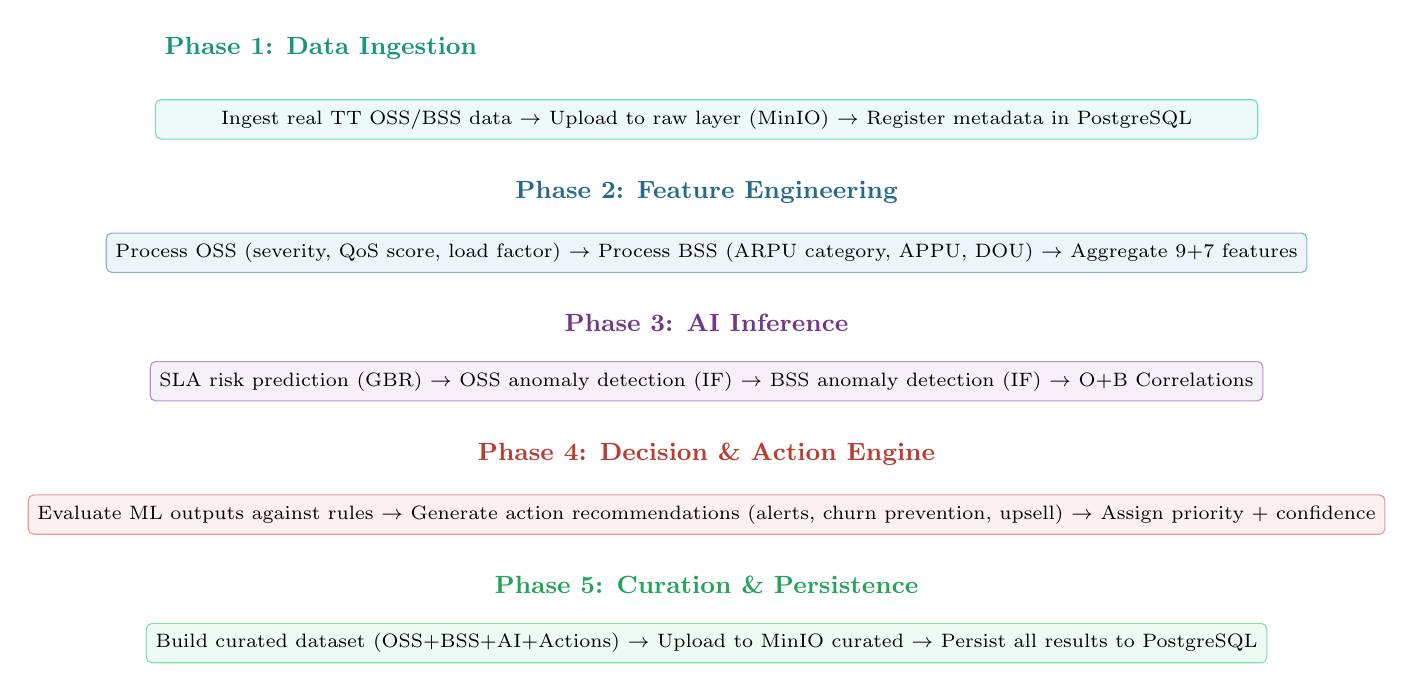
\begin{tikzpicture}[
  step/.style={rectangle,rounded corners=2pt,minimum width=14cm,minimum height=0.5cm,
    draw=#1!60,fill=#1!8,font=\scriptsize,align=left,text=black},
  phase/.style={font=\small\bfseries,text=#1!80!black,anchor=west},
  node distance=0.12cm,
]
  \node[phase=cemteal] (p1) at (0,0) {Phase 1: Data Ingestion};
  \node[step=cemteal,below=0.25cm of p1,anchor=north west] (s1) at (0,-0.4) {
    Ingest real TT OSS/BSS data $\to$ Upload to raw layer (MinIO) $\to$ Register metadata in PostgreSQL};
  \node[phase=ossblue,below=0.4cm of s1] (p2) {Phase 2: Feature Engineering};
  \node[step=ossblue,below=0.25cm of p2] (s2) {
    Process OSS (severity, QoS score, load factor) $\to$ Process BSS (ARPU category, APPU, DOU) $\to$ Aggregate 9+7 features};
  \node[phase=aiviolet,below=0.4cm of s2] (p3) {Phase 3: AI Inference};
  \node[step=aiviolet,below=0.25cm of p3] (s3) {
    SLA risk prediction (GBR) $\to$ OSS anomaly detection (IF) $\to$ BSS anomaly detection (IF) $\to$ O+B Correlations};
  \node[phase=actionred,below=0.4cm of s3] (p4) {Phase 4: Decision \& Action Engine};
  \node[step=actionred,below=0.25cm of p4] (s4) {
    Evaluate ML outputs against rules $\to$ Generate action recommendations (alerts, churn prevention, upsell) $\to$ Assign priority + confidence};
  \node[phase=bssgreen,below=0.4cm of s4] (p5) {Phase 5: Curation \& Persistence};
  \node[step=bssgreen,below=0.25cm of p5] (s5) {
    Build curated dataset (OSS+BSS+AI+Actions) $\to$ Upload to MinIO curated $\to$ Persist all results to PostgreSQL};
\end{tikzpicture}}%
\caption{5-phase pipeline execution flow --- from ingestion to autonomous action.}
\label{fig:pipeline}
\end{figure}

\section{Decision \& Action Engine (Phase 4)}

The Action Engine is what elevates the system from passive analytics to an autonomous agent. It evaluates ML outputs against configurable business rules and generates actionable recommendations:

\begin{table}[H]
\centering\small
\caption{Action rules --- autonomous decision logic.}
\begin{tabularx}{\textwidth}{@{}llXl@{}}
\toprule
\textbf{Trigger Condition} & \textbf{Action Type} & \textbf{Description} & \textbf{Priority} \\
\midrule
SLA risk $> 0.7$ & Proactive Alert & Network degradation warning to NOC with affected cells and predicted impact & Critical \\
SLA risk $\in [0.4, 0.7]$ & Watch Alert & Monitoring advisory with trend direction & Medium \\
OSS anomaly + correlated revenue drop & Churn Prevention & Trigger retention campaign for affected subscriber segment & High \\
BSS anomaly (revenue spike) + healthy network & Upsell Trigger & Recommend premium plan upgrade for high-usage segment & Medium \\
Significant O+B correlation ($p < 0.05$) & Insight Report & Cross-domain insight for CVM strategy team & Low \\
Multiple anomalies, same region & Escalation Ticket & Auto-create incident ticket for NOC + CVM joint review & Critical \\
\bottomrule
\end{tabularx}
\end{table}

Each recommendation is persisted with: action type, target (region/segment/cell), confidence score, priority level, human-readable explanation, and status (pending/approved/executed/dismissed).

\section{Three-Layer Data Lake}

\begin{figure}[H]
\centering
\resizebox{\textwidth}{!}{%
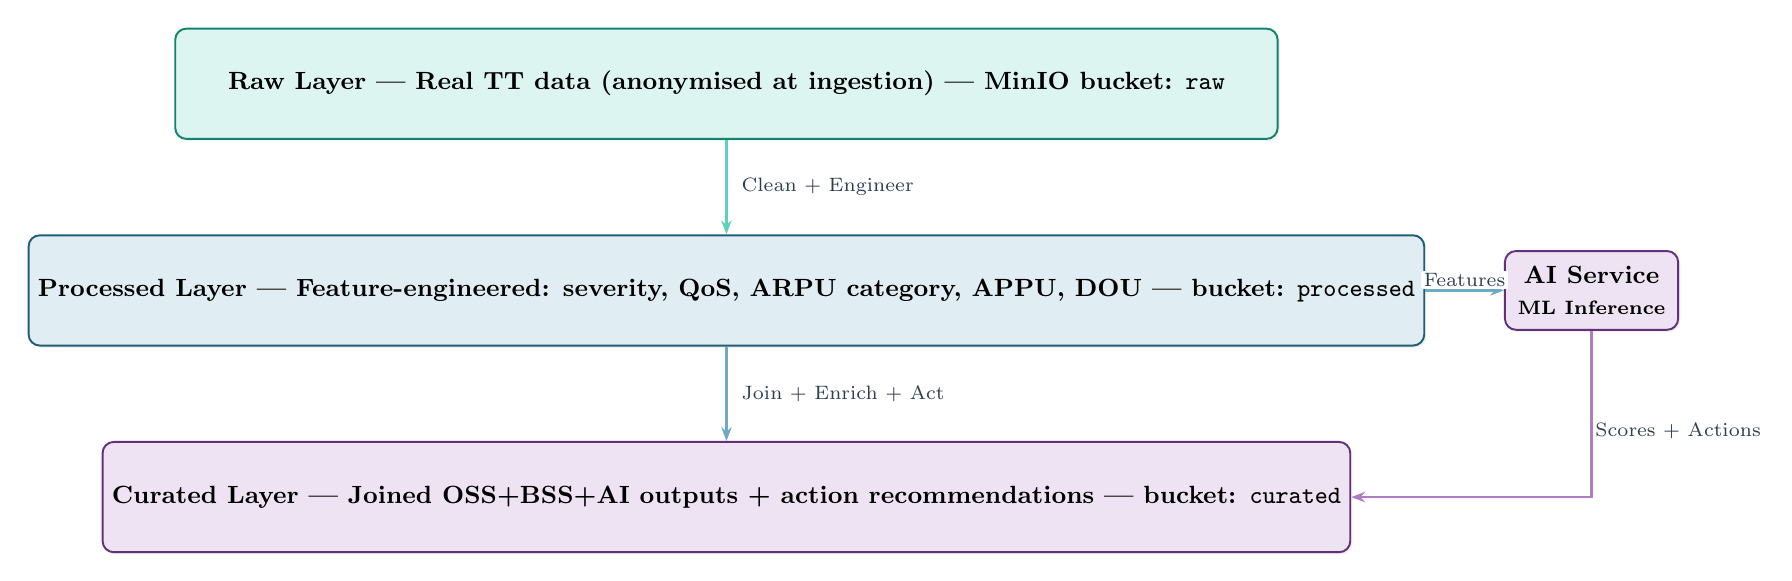
\begin{tikzpicture}[node distance=1.2cm]
  \node[service=cemteal,minimum width=14cm,minimum height=1.4cm] (raw) {
    \textbf{Raw Layer} --- Real TT data (anonymised at ingestion) --- MinIO bucket: \texttt{raw}};
  \node[service=ossblue,minimum width=14cm,minimum height=1.4cm,below=of raw] (proc) {
    \textbf{Processed Layer} --- Feature-engineered: severity, QoS, ARPU category, APPU, DOU --- bucket: \texttt{processed}};
  \node[service=aiviolet,minimum width=14cm,minimum height=1.4cm,below=of proc] (cur) {
    \textbf{Curated Layer} --- Joined OSS+BSS+AI outputs + action recommendations --- bucket: \texttt{curated}};
  \node[service=aiviolet,right=1cm of proc,minimum width=2.2cm] (aiside) {
    \textbf{AI Service}\\{\scriptsize ML Inference}};
  \draw[myarrow=cemteal!70,line width=1pt] (raw) -- (proc) node[arrlabel,midway,right,xshift=4pt] {Clean + Engineer};
  \draw[myarrow=ossblue!70,line width=1pt] (proc) -- (cur) node[arrlabel,midway,right,xshift=4pt] {Join + Enrich + Act};
  \draw[myarrow=ossblue!70] (proc) -- (aiside) node[arrlabel,midway,above] {Features};
  \draw[myarrow=aiviolet!70] (aiside) |- (cur) node[arrlabel,pos=0.3,right] {Scores + Actions};
\end{tikzpicture}}%
\caption{Three-layer data lake: Raw $\to$ Processed $\to$ Curated (with actions).}
\label{fig:datalake}
\end{figure}

% =============================================================================
%  CHAPTER 3 --- INDUSTRIAL CONTEXT
% =============================================================================
\chapter{Industrial Context}

\section{The Huawei Ecosystem}

\begin{figure}[H]
\centering
\resizebox{0.95\textwidth}{!}{%
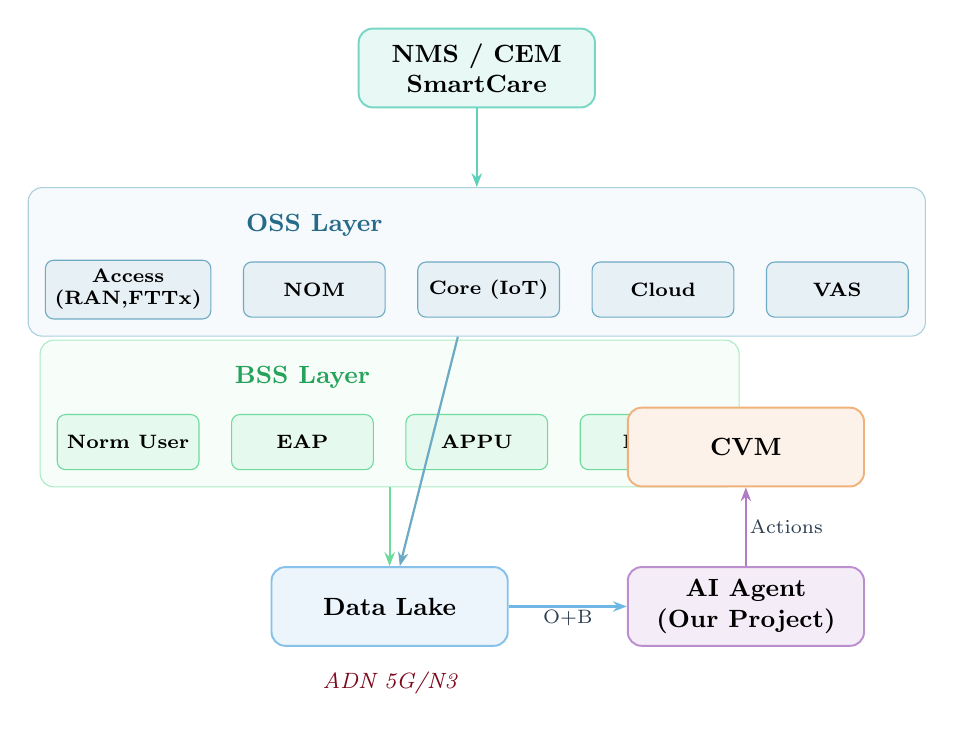
\begin{tikzpicture}[
  node distance=0.3cm and 0.4cm,
  ossbox/.style={rectangle,rounded corners=3pt,minimum width=1.8cm,minimum height=0.7cm,
    draw=ossblue!70,fill=ossblue!12,font=\scriptsize\bfseries,align=center},
  bssbox/.style={rectangle,rounded corners=3pt,minimum width=1.8cm,minimum height=0.7cm,
    draw=bssgreen!70,fill=bssgreen!12,font=\scriptsize\bfseries,align=center},
  bigbox/.style={rectangle,rounded corners=5pt,minimum width=3cm,minimum height=1cm,
    draw=#1!60,fill=#1!10,font=\small\bfseries,align=center,line width=0.7pt},
]
  \node[ossbox] (access) {Access\\(RAN,FTTx)};
  \node[ossbox,right=of access] (nom) {NOM};
  \node[ossbox,right=of nom] (core) {Core (IoT)};
  \node[ossbox,right=of core] (cloud) {Cloud};
  \node[ossbox,right=of cloud] (vas) {VAS};
  \node[above=0.2cm of nom,font=\small\bfseries,text=ossblue!80!black] (osslbl) {OSS Layer};
  \begin{scope}[on background layer]
    \node[fit=(access)(nom)(core)(cloud)(vas)(osslbl),
      draw=ossblue!40,fill=ossblue!4,rounded corners=5pt,inner sep=6pt] (ossgrp) {};
  \end{scope}
  \node[bssbox,below=1.2cm of access] (nu) {Norm User};
  \node[bssbox,right=of nu] (eap) {EAP};
  \node[bssbox,right=of eap] (appu) {APPU};
  \node[bssbox,right=of appu] (dou) {DOU};
  \node[above=0.2cm of eap,font=\small\bfseries,text=bssgreen!80!black] (bsslbl) {BSS Layer};
  \begin{scope}[on background layer]
    \node[fit=(nu)(eap)(appu)(dou)(bsslbl),
      draw=bssgreen!40,fill=bssgreen!4,rounded corners=5pt,inner sep=6pt] (bssgrp) {};
  \end{scope}
  \node[bigbox=cemteal,above=1cm of ossgrp] (nms) {\textbf{NMS / CEM}\\SmartCare};
  \node[bigbox=datalake,below=1cm of bssgrp] (lake) {\textbf{Data Lake}};
  \node[bigbox=aiviolet,right=1.5cm of lake] (ag) {\textbf{AI Agent}\\(Our Project)};
  \node[bigbox=cvmorange,above=1cm of ag] (cvm) {\textbf{CVM}};
  \draw[myarrow=cemteal!70] (nms) -- (ossgrp);
  \draw[myarrow=ossblue!70] (ossgrp) -- (lake);
  \draw[myarrow=bssgreen!70] (bssgrp) -- (lake);
  \draw[myarrow=datalake!70] (lake) -- (ag) node[arrlabel,midway,below] {O+B};
  \draw[myarrow=aiviolet!70] (ag) -- (cvm) node[arrlabel,midway,right] {Actions};
  \node[below=0.2cm of lake,font=\footnotesize\itshape,text=huaweired!60!black] {ADN 5G/N3};
\end{tikzpicture}}%
\caption{Huawei NMS/CEM/OSS/BSS ecosystem with AI Agent positioning.}
\label{fig:huawei-stack}
\end{figure}

\section{ADN Autonomy Levels}

\begin{figure}[H]
\centering
\resizebox{0.85\textwidth}{!}{%
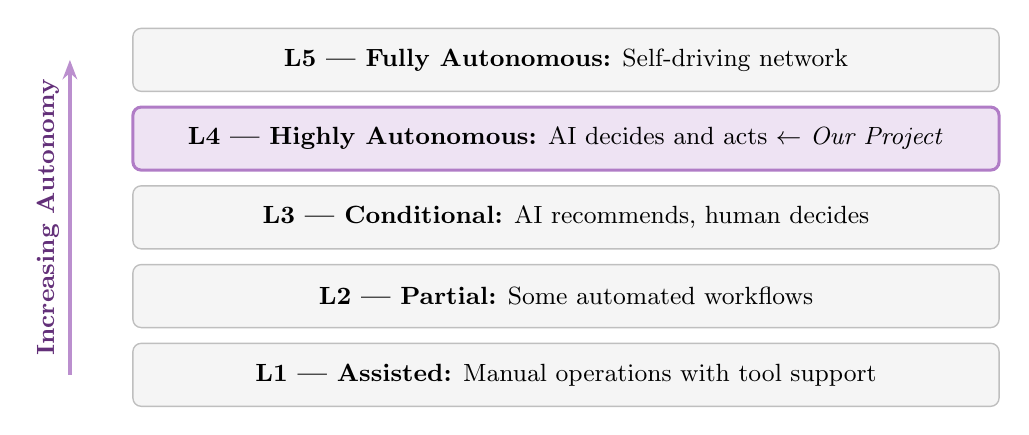
\begin{tikzpicture}[
  level/.style={rectangle,rounded corners=3pt,minimum width=11cm,minimum height=0.8cm,
    font=\small,align=center,line width=0.5pt},
]
  \node[level,draw=gray!50,fill=gray!8] (l1) at (0,0)
    {\textbf{L1 --- Assisted:} Manual operations with tool support};
  \node[level,draw=gray!50,fill=gray!8] (l2) at (0,1)
    {\textbf{L2 --- Partial:} Some automated workflows};
  \node[level,draw=gray!50,fill=gray!8] (l3) at (0,2)
    {\textbf{L3 --- Conditional:} AI recommends, human decides};
  \node[level,draw=aiviolet!70,fill=aiviolet!15,line width=1.1pt] (l4) at (0,3)
    {\textbf{L4 --- Highly Autonomous:} AI decides and acts $\leftarrow$ \textit{Our Project}};
  \node[level,draw=gray!50,fill=gray!8] (l5) at (0,4)
    {\textbf{L5 --- Fully Autonomous:} Self-driving network};
  \draw[-{Stealth[length=7pt]},line width=1.2pt,aiviolet!60] (-6.3,0) -- (-6.3,4)
    node[midway,rotate=90,above,font=\small\bfseries,text=aiviolet!70!black] {Increasing Autonomy};
\end{tikzpicture}}%
\caption{Huawei ADN levels --- project targets L4 (Highly Autonomous).}
\label{fig:adn}
\end{figure}

\noindent\textbf{Why L4, not L3?} At L3 the system only recommends --- a human must approve every action. Our agent goes further: it autonomously generates and triggers actions (alerts, churn prevention, upsell campaigns) based on ML outputs and business rules. Human oversight is reserved for critical escalations only, not for routine decisions. This is the definition of L4: \textit{AI decides and acts; humans handle edge cases.}

% =============================================================================
%  CHAPTER 4 --- AI MODELS
% =============================================================================
\chapter{AI Models \& Intelligence Layer}

\section{Model Overview}

\begin{figure}[H]
\centering
\resizebox{\textwidth}{!}{%
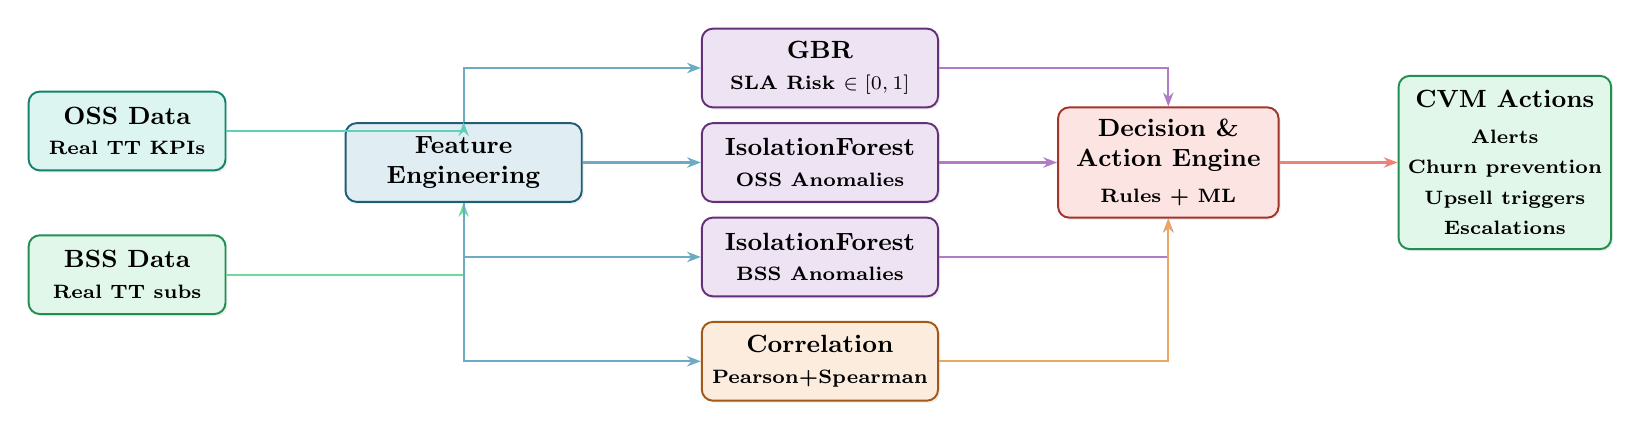
\begin{tikzpicture}[node distance=1.2cm and 1.5cm]
  \node[service=cemteal,minimum width=2.5cm] (oss) {OSS Data\\{\scriptsize Real TT KPIs}};
  \node[service=bssgreen,minimum width=2.5cm,below=0.8cm of oss] (bss) {BSS Data\\{\scriptsize Real TT subs}};
  \node[service=ossblue,right=1.5cm of oss,yshift=-0.4cm,minimum width=3cm] (feat) {
    \textbf{Feature}\\
    \textbf{Engineering}};
  \node[service=aiviolet,right=1.5cm of feat,yshift=1.2cm,minimum width=3cm] (gbr) {
    \textbf{GBR}\\{\scriptsize SLA Risk $\in[0,1]$}};
  \node[service=aiviolet,right=1.5cm of feat,minimum width=3cm] (ifoss) {
    \textbf{IsolationForest}\\{\scriptsize OSS Anomalies}};
  \node[service=aiviolet,right=1.5cm of feat,yshift=-1.2cm,minimum width=3cm] (ifbss) {
    \textbf{IsolationForest}\\{\scriptsize BSS Anomalies}};
  \node[service=cvmorange,below=0.3cm of ifbss,minimum width=3cm] (corr) {
    \textbf{Correlation}\\{\scriptsize Pearson+Spearman}};
  \node[service=actionred,right=1.5cm of ifoss,minimum width=2.8cm,minimum height=1.4cm] (engine) {
    \textbf{Decision \&}\\
    \textbf{Action Engine}\\[2pt]
    {\scriptsize Rules + ML}};
  \node[service=bssgreen,right=1.5cm of engine,minimum width=2.5cm,minimum height=2.2cm] (out) {
    \textbf{CVM Actions}\\[2pt]
    {\scriptsize Alerts}\\
    {\scriptsize Churn prevention}\\
    {\scriptsize Upsell triggers}\\
    {\scriptsize Escalations}};
  \draw[myarrow=cemteal!70] (oss) -| (feat);
  \draw[myarrow=bssgreen!70] (bss) -| (feat);
  \draw[myarrow=ossblue!70] (feat) |- (gbr);
  \draw[myarrow=ossblue!70] (feat) -- (ifoss);
  \draw[myarrow=ossblue!70] (feat) |- (ifbss);
  \draw[myarrow=ossblue!70] (feat) |- (corr);
  \draw[myarrow=aiviolet!70] (gbr) -| (engine);
  \draw[myarrow=aiviolet!70] (ifoss) -- (engine);
  \draw[myarrow=aiviolet!70] (ifbss) -| (engine);
  \draw[myarrow=cvmorange!70] (corr) -| (engine);
  \draw[myarrow=actionred!70,line width=1pt] (engine) -- (out);
\end{tikzpicture}}%
\caption{ML pipeline: Data $\to$ Features $\to$ 3 Models + Correlation $\to$ Decision Engine $\to$ CVM Actions.}
\label{fig:ml-pipeline}
\end{figure}

\begin{table}[H]
\centering\small
\caption{Model inventory.}
\begin{tabularx}{\textwidth}{@{}llllX@{}}
\toprule
\textbf{Model} & \textbf{Algorithm} & \textbf{Type} & \textbf{Features} & \textbf{Output} \\
\midrule
SLA Risk     & GradientBoostingRegressor & Supervised   & 9 OSS agg.  & Risk $\in[0,1]$ + importances \\
OSS Anomaly  & IsolationForest           & Unsupervised & 5 per-record & Anomaly flag + severity \\
BSS Anomaly  & IsolationForest           & Unsupervised & 7 per-record & Anomaly flag + severity \\
Correlation  & Pearson + Spearman        & Statistical  & 5 OSS--BSS pairs & 10 coefficients + p-values \\
\midrule
\textbf{Action Engine} & \textbf{Rule-based + ML} & \textbf{Autonomous} & \textbf{All outputs} & \textbf{Typed recommendations + priority} \\
\bottomrule
\end{tabularx}
\end{table}

\section{SLA Risk Prediction (GBR)}

\textbf{Input:} 9 aggregate OSS features per time window per region:
$$\mathbf{x} = \begin{bmatrix} \bar{T} & \sigma_T & \bar{L} & \sigma_L & L_{\max} & \bar{P} & P_{\max} & \bar{U} & \bar{S}\end{bmatrix}$$

\textbf{Risk label} (domain-knowledge formula):
\begin{align*}
y &= \mathrm{clip}\!\left(\tfrac{\bar{L}-20}{60},0,0.35\right)
   + \mathrm{clip}\!\left(\tfrac{L_{\max}-30}{70},0,0.25\right)
   + \mathrm{clip}\!\left(\tfrac{\bar{P}}{4},0,0.25\right)\\
  &+ \mathrm{clip}\!\left(\tfrac{P_{\max}}{6},0,0.15\right)
   + \mathrm{clip}\!\left(\tfrac{60-\bar{T}}{100},0,0.20\right) + \epsilon
\end{align*}

\textbf{Feature importances} (v2.0): \texttt{mean\_latency} dominates at 0.69.

\begin{figure}[H]
\centering
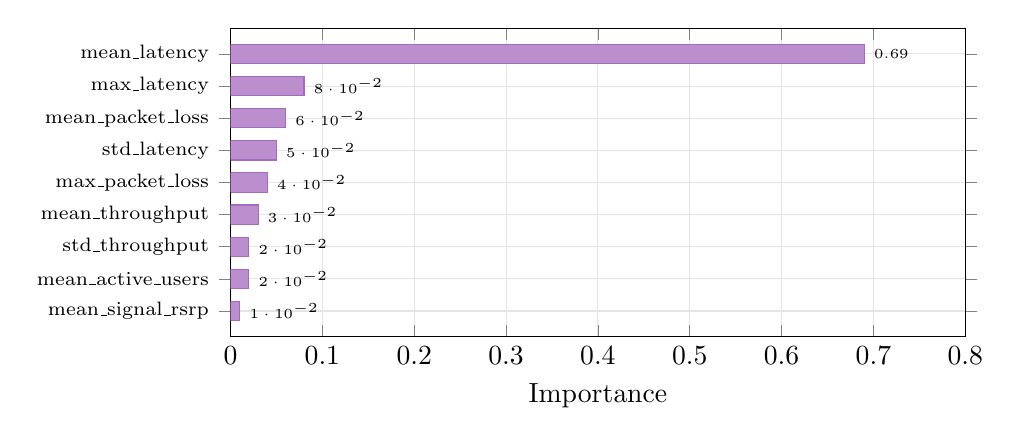
\begin{tikzpicture}
\begin{axis}[
  xbar, width=0.9\textwidth, height=5.5cm,
  xlabel={Importance}, symbolic y coords={
    {mean\_signal\_rsrp},{mean\_active\_users},{std\_throughput},{mean\_throughput},
    {max\_packet\_loss},{std\_latency},{mean\_packet\_loss},{max\_latency},{mean\_latency}},
  ytick=data, y tick label style={font=\scriptsize},
  xmin=0, xmax=0.8, bar width=7pt,
  nodes near coords, nodes near coords align={horizontal},
  every node near coord/.append style={font=\tiny},
  enlarge y limits=0.1, grid=major, grid style={gray!20},
]
\addplot[fill=aiviolet!60,draw=aiviolet!80] coordinates {
  (0.69,{mean\_latency}) (0.08,{max\_latency}) (0.06,{mean\_packet\_loss})
  (0.05,{std\_latency}) (0.04,{max\_packet\_loss}) (0.03,{mean\_throughput})
  (0.02,{std\_throughput}) (0.02,{mean\_active\_users}) (0.01,{mean\_signal\_rsrp})
};
\end{axis}
\end{tikzpicture}
\caption{Feature importances --- GBR v2.0. \texttt{mean\_latency} = 0.69.}
\label{fig:feat-imp}
\end{figure}

\section{Anomaly Detection (IsolationForest)}

\textbf{OSS} (5 features): throughput, latency, packet loss, active users, RSRP.\\
\textbf{BSS} (7 features): revenue, data usage, voice, SMS, churn risk, APPU, DOU.

Anomaly severity normalised to $[0,1]$:
$$\text{severity}_i = 1 - \frac{s_i - s_{\min}}{s_{\max} - s_{\min} + \epsilon}$$

\section{O+B Correlation Engine}

\begin{table}[H]
\centering\small
\caption{OSS--BSS correlation pairs.}
\begin{tabular}{@{}lll@{}}
\toprule
\textbf{OSS Metric} & \textbf{BSS Metric} & \textbf{Expected} \\
\midrule
throughput\_mbps  & revenue\_tnd   & Positive \\
latency\_ms       & revenue\_tnd   & Negative \\
packet\_loss\_pct & churn\_risk    & Positive \\
latency\_ms       & data\_used\_gb & Negative \\
signal\_rsrp\_dbm & revenue\_tnd   & Positive \\
\bottomrule
\end{tabular}
\end{table}

% =============================================================================
%  CHAPTER 5 --- DATA STRATEGY
% =============================================================================
\chapter{Data Strategy}

\section{Data Sources}

\begin{table}[H]
\centering\small
\caption{Data sources.}
\begin{tabularx}{\textwidth}{@{}lllX@{}}
\toprule
\textbf{Source} & \textbf{Domain} & \textbf{Format} & \textbf{Content} \\
\midrule
Tunisie Telecom & BSS & CSV/Excel & Subscriber profiles, ARPU, DOU, churn, revenue \\
Tunisie Telecom & OSS & CSV/JSON  & Cell KPIs: throughput, latency, packet loss, users \\
Huawei SmartCare & CEM & CSV/JSON  & KQI, CEI, demarcation results \\
Synthetic       & Both & In-memory & Fallback when no real data available \\
\bottomrule
\end{tabularx}
\end{table}

\section{Data Ingestion Flow}

\begin{figure}[H]
\centering
\resizebox{\textwidth}{!}{%
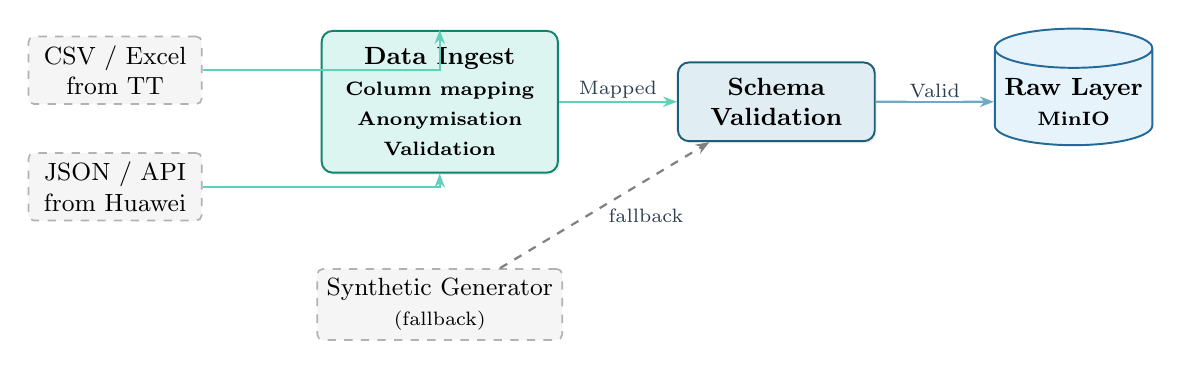
\begin{tikzpicture}[node distance=1cm and 1.5cm]
  \node[external,minimum width=2.2cm] (csv) {CSV / Excel\\from TT};
  \node[external,minimum width=2.2cm,below=0.6cm of csv] (json) {JSON / API\\from Huawei};
  \node[service=cemteal,right=1.5cm of csv,yshift=-0.4cm,minimum width=3cm,minimum height=1.8cm] (ingest) {
    \textbf{Data Ingest}\\{\scriptsize Column mapping}\\{\scriptsize Anonymisation}\\{\scriptsize Validation}};
  \node[service=ossblue,right=1.5cm of ingest,minimum width=2.5cm] (validate) {
    \textbf{Schema}\\
    \textbf{Validation}};
  \node[datastore=datalake,right=1.5cm of validate] (rawlk) {\textbf{Raw Layer}\\{\scriptsize MinIO}};
  \draw[myarrow=cemteal!70] (csv) -| (ingest);
  \draw[myarrow=cemteal!70] (json) -| (ingest);
  \draw[myarrow=cemteal!70] (ingest) -- (validate) node[arrlabel,midway,above] {Mapped};
  \draw[myarrow=ossblue!70] (validate) -- (rawlk) node[arrlabel,midway,above] {Valid};
  \node[external,below=1.2cm of ingest,minimum width=3cm] (synth) {Synthetic Generator\\{\scriptsize (fallback)}};
  \draw[myarrow=gray,dashed] (synth) -- (validate) node[arrlabel,midway,below right] {\scriptsize fallback};
\end{tikzpicture}}%
\caption{Data ingestion flow --- real TT data is mapped, anonymised, and validated.}
\label{fig:ingestion}
\end{figure}

\section{Anonymisation}

\begin{table}[H]
\centering\small
\caption{Anonymisation applied to incoming TT data.}
\begin{tabularx}{\textwidth}{@{}llX@{}}
\toprule
\textbf{Field} & \textbf{Method} & \textbf{Rationale} \\
\midrule
MSISDN  & SHA-256 hash + salt & Linkage without exposing phone numbers \\
Name/Address & Stripped           & Not needed for analysis \\
Location & Gouvernorat only     & No GPS coordinates \\
Cell IDs & Optional opaque map  & Anonymise if TT requires \\
\bottomrule
\end{tabularx}
\end{table}

% =============================================================================
%  CHAPTER 6 --- CLOUD DEPLOYMENT
% =============================================================================
\chapter{Cloud Deployment (HCS)}

\section{Local $\to$ HCS Mapping}

\begin{figure}[H]
\centering
\resizebox{\textwidth}{!}{%
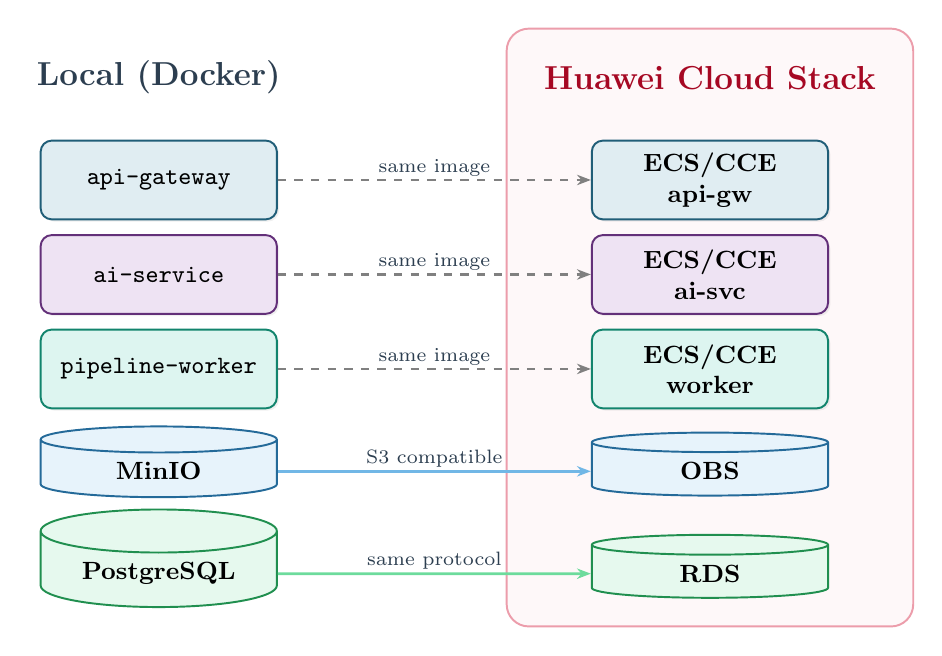
\begin{tikzpicture}[node distance=1.2cm and 3cm]
  \node[font=\large\bfseries,text=darkbg] (lt) at (0,4.5) {Local (Docker)};
  \node[service=ossblue,minimum width=3cm]  (la) at (0,3.2) {\texttt{api-gateway}};
  \node[service=aiviolet,minimum width=3cm] (li) at (0,2)   {\texttt{ai-service}};
  \node[service=cemteal,minimum width=3cm]  (lw) at (0,0.8) {\texttt{pipeline-worker}};
  \node[datastore=datalake,minimum width=3cm,minimum height=0.8cm] (lm) at (0,-0.5) {\textbf{MinIO}};
  \node[datastore=bssgreen,minimum width=3cm,minimum height=0.8cm] (lp) at (0,-1.8) {\textbf{PostgreSQL}};
  \node[font=\large\bfseries,text=huaweired!80!black] (ht) at (7,4.5) {Huawei Cloud Stack};
  \node[service=ossblue,minimum width=3cm]  (ha) at (7,3.2) {\textbf{ECS/CCE}\\api-gw};
  \node[service=aiviolet,minimum width=3cm] (hi) at (7,2)   {\textbf{ECS/CCE}\\ai-svc};
  \node[service=cemteal,minimum width=3cm]  (hw) at (7,0.8) {\textbf{ECS/CCE}\\worker};
  \node[datastore=datalake,minimum width=3cm,minimum height=0.8cm] (ho) at (7,-0.5) {\textbf{OBS}};
  \node[datastore=bssgreen,minimum width=3cm,minimum height=0.8cm] (hr) at (7,-1.8) {\textbf{RDS}};
  \begin{scope}[on background layer]
    \node[fit=(ht)(ha)(hi)(hw)(ho)(hr),draw=huaweired!40,fill=huaweired!3,
      rounded corners=8pt,inner sep=10pt,line width=0.7pt] {};
  \end{scope}
  \draw[myarrow=gray,line width=1pt,dashed] (la) -- (ha) node[arrlabel,midway,above] {same image};
  \draw[myarrow=gray,line width=1pt,dashed] (li) -- (hi) node[arrlabel,midway,above] {same image};
  \draw[myarrow=gray,line width=1pt,dashed] (lw) -- (hw) node[arrlabel,midway,above] {same image};
  \draw[myarrow=datalake!70,line width=1pt] (lm) -- (ho) node[arrlabel,midway,above] {S3 compatible};
  \draw[myarrow=bssgreen!70,line width=1pt] (lp) -- (hr) node[arrlabel,midway,above] {same protocol};
\end{tikzpicture}}%
\caption{Docker Compose $\to$ HCS mapping.}
\label{fig:hcs}
\end{figure}

\section{HCS Target Architecture}

\begin{figure}[H]
\centering
\resizebox{0.95\textwidth}{!}{%
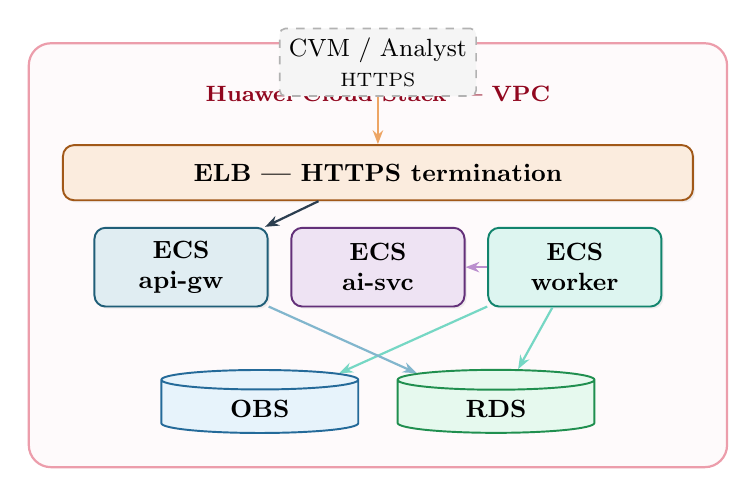
\begin{tikzpicture}[node distance=1cm and 1.5cm]
  \node[font=\footnotesize\bfseries,text=huaweired!70!black] (vpc) at (3.5,5) {Huawei Cloud Stack --- VPC};
  \node[service=cvmorange,minimum width=8cm,minimum height=0.7cm] (elb) at (3.5,4) {
    \textbf{ELB} --- HTTPS termination};
  \node[service=ossblue,minimum width=2.2cm] (api) at (1,2.8) {\textbf{ECS}\\api-gw};
  \node[service=aiviolet,minimum width=2.2cm] (ai)  at (3.5,2.8) {\textbf{ECS}\\ai-svc};
  \node[service=cemteal,minimum width=2.2cm] (wk)  at (6,2.8) {\textbf{ECS}\\worker};
  \node[datastore=datalake,minimum width=2.5cm,minimum height=0.8cm] (obs) at (2,1) {\textbf{OBS}};
  \node[datastore=bssgreen,minimum width=2.5cm,minimum height=0.8cm] (rds) at (5,1) {\textbf{RDS}};
  \begin{scope}[on background layer]
    \node[fit=(vpc)(elb)(api)(ai)(wk)(obs)(rds),draw=huaweired!40,fill=huaweired!2,
      rounded corners=8pt,inner sep=12pt,line width=0.8pt] {};
  \end{scope}
  \draw[myarrow] (elb) -- (api);
  \draw[myarrow=aiviolet!60] (wk) -- (ai);
  \draw[myarrow=cemteal!60] (wk) -- (obs);
  \draw[myarrow=cemteal!60] (wk) -- (rds);
  \draw[myarrow=ossblue!60] (api) -- (rds);
  \node[external,above=0.6cm of elb] (ext) {CVM / Analyst\\{\scriptsize HTTPS}};
  \draw[myarrow=cvmorange!70,line width=1pt] (ext) -- (elb);
\end{tikzpicture}}%
\caption{HCS target deployment: VPC, ELB, ECS, OBS, RDS.}
\label{fig:hcs-target}
\end{figure}

% =============================================================================
%  CHAPTER 7 --- DATABASE \& API
% =============================================================================
\chapter{Database \& API}

\section{Entity-Relationship Diagram (8 Tables)}

\begin{figure}[H]
\centering
\resizebox{\textwidth}{!}{%
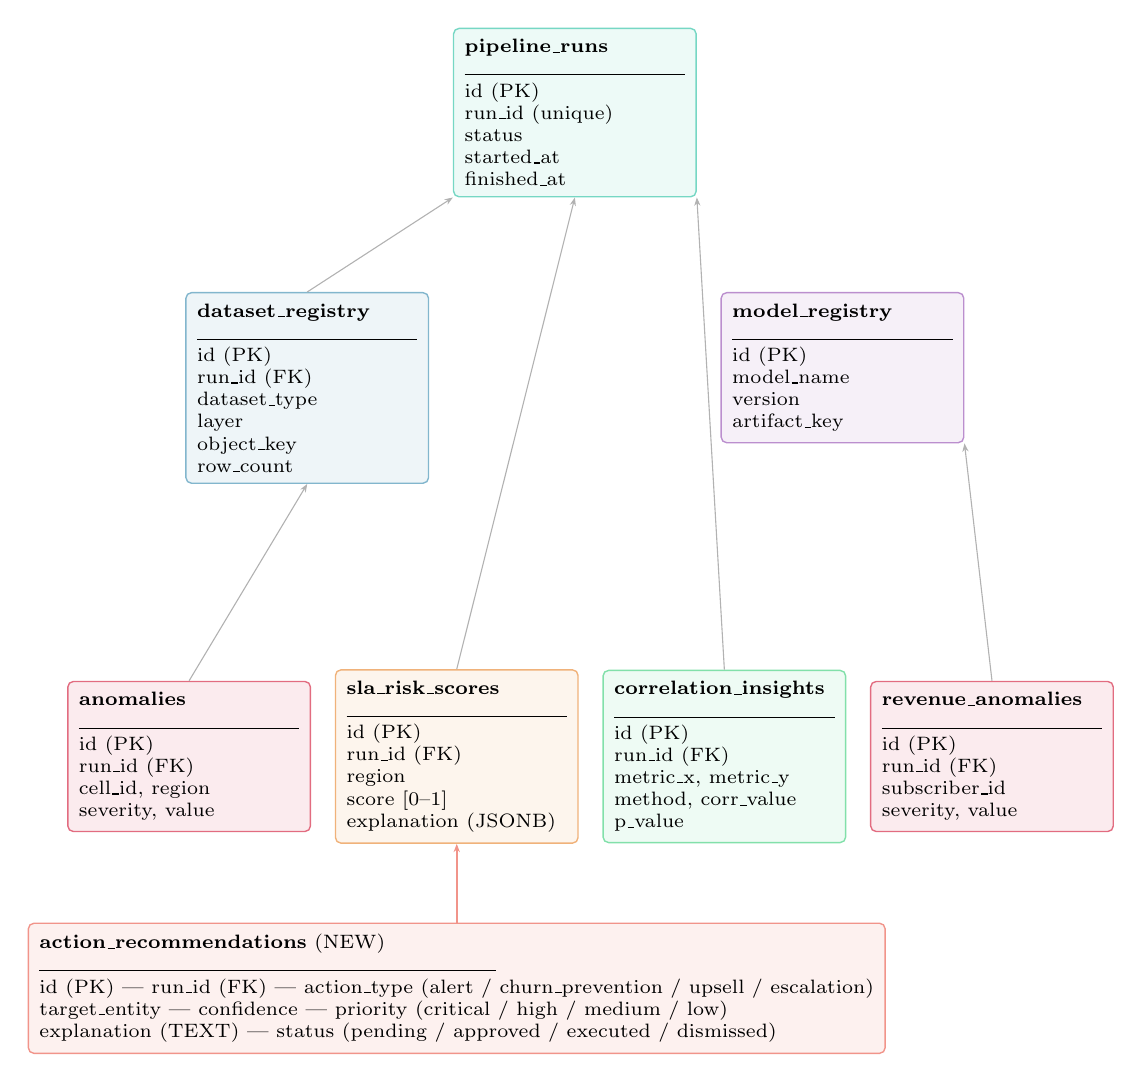
\begin{tikzpicture}[
  entity/.style={rectangle,rounded corners=2pt,draw=#1!60,fill=#1!8,
    minimum width=3cm,font=\scriptsize,align=left,inner sep=4pt,line width=0.5pt},
  entity/.default={darkbg},
  fk/.style={-{Stealth[length=3pt]},draw=gray!60,line width=0.4pt},
  node distance=1cm and 1.5cm,
]
  \node[entity=cemteal] (runs) {
    \textbf{pipeline\_runs}\\
    \rule{2.8cm}{0.2pt}\\id (PK)\\run\_id (unique)\\status\\started\_at\\finished\_at};
  \node[entity=ossblue,below left=1.2cm and 0.3cm of runs] (ds) {
    \textbf{dataset\_registry}\\
    \rule{2.8cm}{0.2pt}\\id (PK)\\run\_id (FK)\\dataset\_type\\layer\\object\_key\\row\_count};
  \node[entity=aiviolet,below right=1.2cm and 0.3cm of runs] (mdl) {
    \textbf{model\_registry}\\
    \rule{2.8cm}{0.2pt}\\id (PK)\\model\_name\\version\\artifact\_key};
  \node[entity=huaweired,below=2.5cm of ds,xshift=-1.5cm] (anom) {
    \textbf{anomalies}\\
    \rule{2.8cm}{0.2pt}\\id (PK)\\run\_id (FK)\\cell\_id, region\\severity, value};
  \node[entity=cvmorange,right=0.3cm of anom] (sla) {
    \textbf{sla\_risk\_scores}\\
    \rule{2.8cm}{0.2pt}\\id (PK)\\run\_id (FK)\\region\\score [0--1]\\explanation (JSONB)};
  \node[entity=bssgreen,right=0.3cm of sla] (corr) {
    \textbf{correlation\_insights}\\
    \rule{2.8cm}{0.2pt}\\id (PK)\\run\_id (FK)\\metric\_x, metric\_y\\method, corr\_value\\p\_value};
  \node[entity=huaweired,right=0.3cm of corr] (rev) {
    \textbf{revenue\_anomalies}\\
    \rule{2.8cm}{0.2pt}\\id (PK)\\run\_id (FK)\\subscriber\_id\\severity, value};
  \node[entity=actionred,below=1cm of sla,minimum width=6cm] (act) {
    \textbf{action\_recommendations} (NEW)\\
    \rule{5.8cm}{0.2pt}\\id (PK) | run\_id (FK) | action\_type (alert / churn\_prevention / upsell / escalation)\\
    target\_entity | confidence | priority (critical / high / medium / low)\\
    explanation (TEXT) | status (pending / approved / executed / dismissed)};
  \draw[fk] (ds.north) -- (runs.south west);
  \draw[fk] (anom.north) -- (ds.south);
  \draw[fk] (sla.north) -- (runs.south);
  \draw[fk] (corr.north) -- (runs.south east);
  \draw[fk] (rev.north) -- (mdl.south east);
  \draw[fk,actionred!60,line width=0.6pt] (act.north) -- (sla.south);
\end{tikzpicture}}%
\caption{ER diagram --- 8 PostgreSQL tables (incl.\ action\_recommendations).}
\label{fig:er}
\end{figure}

\section{REST API Endpoints}

\begin{table}[H]
\centering\small
\caption{API Gateway endpoints (port 8000).}
\begin{tabularx}{\textwidth}{@{}llX@{}}
\toprule
\textbf{Method} & \textbf{Path} & \textbf{Description} \\
\midrule
GET & \texttt{/health}            & Liveness check \\
GET & \texttt{/sla-risk}          & Latest SLA risk score \\
GET & \texttt{/sla-risk/history}  & Last N risk scores \\
GET & \texttt{/anomalies}         & Latest OSS anomalies \\
GET & \texttt{/pipeline-runs}     & Pipeline execution history \\
GET & \texttt{/revenue-anomalies} & BSS revenue anomalies \\
GET & \texttt{/correlation}       & OSS--BSS correlation results \\
GET & \texttt{/actions}           & Pending action recommendations \\
PATCH & \texttt{/actions/\{id\}}  & Approve / dismiss an action \\
\bottomrule
\end{tabularx}
\end{table}

\begin{table}[H]
\centering\small
\caption{AI Service internal endpoints (port 8001).}
\begin{tabularx}{\textwidth}{@{}lllX@{}}
\toprule
\textbf{Method} & \textbf{Path} & \textbf{Model} & \textbf{Output} \\
\midrule
GET  & \texttt{/health}                & ---  & Status + model version \\
POST & \texttt{/infer/sla-risk}        & GBR  & Risk score + feature importances \\
POST & \texttt{/infer/anomaly}         & IF   & Per-record anomaly flag + severity \\
POST & \texttt{/infer/revenue-anomaly} & IF   & Per-record anomaly flag + severity \\
\bottomrule
\end{tabularx}
\end{table}

% =============================================================================
%  CHAPTER 8 --- GAP ANALYSIS
% =============================================================================
\chapter{Gap Analysis \& Positioning}

\begin{figure}[H]
\centering
\resizebox{0.9\textwidth}{!}{%
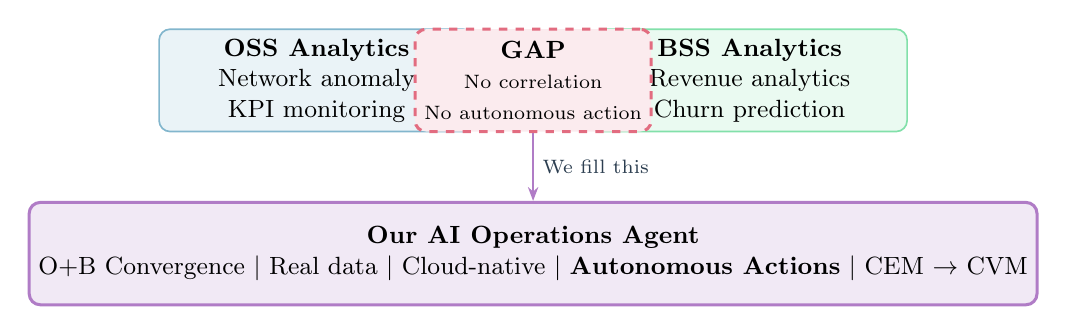
\begin{tikzpicture}[
  gn/.style={rectangle,rounded corners=4pt,minimum width=4cm,minimum height=1.3cm,
    font=\small,align=center,line width=0.6pt},
]
  \node[gn,draw=ossblue!60,fill=ossblue!10] (oss) at (0,0) {
    \textbf{OSS Analytics}\\Network anomaly\\KPI monitoring};
  \node[gn,draw=bssgreen!60,fill=bssgreen!10] (bss) at (5.5,0) {
    \textbf{BSS Analytics}\\Revenue analytics\\Churn prediction};
  \node[gn,draw=huaweired!60,fill=huaweired!8,dashed,line width=1.1pt,
    minimum width=2.5cm] (gap) at (2.75,0) {
    \textbf{GAP}\\{\scriptsize No correlation}\\{\scriptsize No autonomous action}};
  \node[gn,draw=aiviolet!70,fill=aiviolet!12,minimum width=9.5cm,line width=1.1pt] (ours) at (2.75,-2.2) {
    \textbf{Our AI Operations Agent}\\
    O+B Convergence $|$ Real data $|$ Cloud-native $|$ \textbf{Autonomous Actions} $|$ CEM $\to$ CVM};
  \draw[myarrow=aiviolet!70,line width=0.9pt] (gap) -- (ours)
    node[arrlabel,midway,right,xshift=2pt] {We fill this};
\end{tikzpicture}}%
\caption{Gap analysis: our AI Agent bridges the OSS--BSS gap with autonomous actions.}
\label{fig:gap}
\end{figure}

\begin{table}[H]
\centering\small
\caption{Comparison with related approaches.}
\begin{tabularx}{\textwidth}{@{}lXccccc@{}}
\toprule
\textbf{Approach} & \textbf{Focus} & \textbf{Real} & \textbf{O+B} & \textbf{Cloud} & \textbf{Agent} & \textbf{Actions} \\
\midrule
SELFNET        & Self-healing 5G        & No  & No & No  & No  & Part. \\
ETSI ZSM       & Zero-touch mgmt        & Spec& Part.& Yes & Part.& Spec \\
Nokia AVA      & Telecom analytics      & Yes & No & Yes & No  & No \\
SmartCare      & CEM + demarcation      & Yes & Part.& Yes & No  & No \\
Ericsson EOM   & Expert-system ops      & Yes & No & Yes & No  & Part. \\
\textbf{Ours}  & \textbf{CEM--CVM Agent}& \textbf{Yes} & \textbf{Yes} & \textbf{Yes} & \textbf{Yes} & \textbf{Yes} \\
\bottomrule
\end{tabularx}
\end{table}

% =============================================================================
%  CHAPTER 9 --- DELIVERABLES
% =============================================================================
\chapter{Project Deliverables}

\begin{table}[H]
\centering\small
\caption{Complete project deliverables.}
\begin{tabularx}{\textwidth}{@{}llX@{}}
\toprule
\textbf{Category} & \textbf{Deliverable} & \textbf{Description} \\
\midrule
\multirow{5}{*}{Software}
  & Docker Compose stack & 5 containers, one-command deploy \\
  & API Gateway          & 9 REST endpoints incl.\ action management (FastAPI) \\
  & AI Service           & 3 ML models + 4 inference endpoints \\
  & Pipeline Worker      & 5-phase pipeline with Decision \& Action Engine \\
  & Data Lake            & 3-layer MinIO (raw / processed / curated) \\
\midrule
\multirow{4}{*}{Intelligence}
  & SLA Risk Model       & GBR trained on real TT data \\
  & OSS/BSS Anomaly      & 2$\times$ IsolationForest (5+7 features) \\
  & O+B Correlations     & Pearson + Spearman on 5 metric pairs \\
  & Action Engine        & Rule-based autonomous recommendation generator \\
\midrule
\multirow{3}{*}{Actions}
  & Proactive Alerts     & Network degradation warnings (SLA risk $>$ 0.7) \\
  & Churn Prevention     & Retention campaigns for anomaly-affected segments \\
  & Upsell Triggers      & Premium plan recommendations for healthy segments \\
\midrule
\multirow{2}{*}{Data}
  & Anonymised TT data   & Real operator data, schema-mapped \\
  & 8-table PostgreSQL   & Metadata, anomalies, risk, correlations, \textbf{actions} \\
\midrule
\multirow{2}{*}{Cloud}
  & HCS architecture map & MinIO$\to$OBS, PG$\to$RDS, Docker$\to$ECS \\
  & Deployment guide     & Step-by-step HCS deployment \\
\bottomrule
\end{tabularx}
\end{table}

\end{document}
